%%%%%%%%%%%%%%%%%%%%%%%%%%%%%%%%%%%%%%%%%
% Structured General Purpose Assignment
% LaTeX Template
%
% This template has been downloaded from:
% http://www.latextemplates.com
%
% Original author:
% Ted Pavlic (http://www.tedpavlic.com)
%
% Note:
% The \lipsum[#] commands throughout this template generate dummy text
% to fill the template out. These commands should all be removed when 
% writing assignment content.
%
%%%%%%%%%%%%%%%%%%%%%%%%%%%%%%%%%%%%%%%%%

%----------------------------------------------------------------------------------------
%	PACKAGES AND OTHER DOCUMENT CONFIGURATIONS
%----------------------------------------------------------------------------------------

\documentclass{article}

\usepackage{tikz}
\usepackage{fancyhdr} % Required for custom headers
\usepackage{lastpage} % Required to determine the last page for the footer
\usepackage{extramarks} % Required for headers and footers
\usepackage{graphicx} % Required to insert images
\usepackage{lipsum} % Used for inserting dummy 'Lorem ipsum' text into the template
\usepackage{mathtools}
\usepackage{amssymb}

% Margins
\topmargin=-0.45in
\evensidemargin=0in
\oddsidemargin=0in
\textwidth=6.5in
\textheight=9.0in
\headsep=0.25in 

\linespread{1.1} % Line spacing

% Set up the header and footer
\pagestyle{fancy}
\lhead{\hmwkAuthorName} % Top left header
\chead{Discussion enrolled: \hmwkClass\\Discussion Attended: \hmwkClass} % Top center header
\rhead{Page\ \thepage\ of\ \pageref{LastPage}} % Bottom right footer
\cfoot{\hmwkTitle} % Bottom center footer
\renewcommand\headrulewidth{0.4pt} % Size of the header rule
\renewcommand\footrulewidth{0.4pt} % Size of the footer rule


%----------------------------------------------------------------------------------------
%	DOCUMENT STRUCTURE COMMANDS
%	Skip this unless you know what you're doing
%----------------------------------------------------------------------------------------

% Header and footer for when a page split occurs within a problem environment
\newcommand{\enterProblemHeader}[1]{
\nobreak\extramarks{#1}{#1 continued on next page\ldots}\nobreak
\nobreak\extramarks{#1 (continued)}{#1 continued on next page\ldots}\nobreak
}

% Header and footer for when a page split occurs between problem environments
\newcommand{\exitProblemHeader}[1]{
\nobreak\extramarks{#1 (continued)}{#1 continued on next page\ldots}\nobreak
\nobreak\extramarks{#1}{}\nobreak
}

\setcounter{secnumdepth}{0} % Removes default section numbers
\newcounter{homeworkProblemCounter} % Creates a counter to keep track of the number of problems

\newcommand{\homeworkProblemName}{}
\newenvironment{homeworkProblem}[1][Problem \arabic{homeworkProblemCounter}]{ % Makes a new environment called homeworkProblem which takes 1 argument (custom name) but the default is "Problem #"
\stepcounter{homeworkProblemCounter} % Increase counter for number of problems
\renewcommand{\homeworkProblemName}{#1} % Assign \homeworkProblemName the name of the problem
\section{\homeworkProblemName} % Make a section in the document with the custom problem count
\enterProblemHeader{\homeworkProblemName} % Header and footer within the environment
}{
\exitProblemHeader{\homeworkProblemName} % Header and footer after the environment
}

\newcommand{\problemAnswer}[1]{ % Defines the problem answer command with the content as the only argument
\noindent\framebox[\columnwidth][c]{\begin{minipage}{0.98\columnwidth}#1\end{minipage}} % Makes the box around the problem answer and puts the content inside
}

\newcommand{\homeworkSectionName}{}
\newenvironment{homeworkSection}[1]{ % New environment for sections within homework problems, takes 1 argument - the name of the section
\renewcommand{\homeworkSectionName}{#1} % Assign \homeworkSectionName to the name of the section from the environment argument
\subsection{\homeworkSectionName} % Make a subsection with the custom name of the subsection
\enterProblemHeader{\homeworkProblemName\ [\homeworkSectionName]} % Header and footer within the environment
}{
\enterProblemHeader{\homeworkProblemName} % Header and footer after the environment
}
   
%----------------------------------------------------------------------------------------
%	NAME AND CLASS SECTION
%----------------------------------------------------------------------------------------

\newcommand{\hmwkTitle}{Assignment 6} % Assignment title
\newcommand{\hmwkClass}{Section 1D} % Course/class
\newcommand{\hmwkAuthorName}{Prianna \underline{Ahsan}} % Your name


\begin{document}

%----------------------------------------------------------------------------------------
%	PROBLEM 1
%----------------------------------------------------------------------------------------

% To have just one problem per page, simply put a \clearpage after each problem

\begin{homeworkProblem}
An ordered graph G = \{V,E\}, such that V = $\{v_1, v_2, ... ,v_n\}$ is a directed graph with the following properties:\\ 
\setlength\parindent{25pt}
\indent i) $e = \{(v_i, v_j) | i < j\}$ $\forall e \in E.$\\
\indent ii) $\delta_{out}(v)\geq 1$ $\forall v_i, i = 1, 2,..., n-1.$\\
Given an ordered graph G, find the length of the longest path that begins at $v_1$ and ends at $v_n$.\\

\begin{homeworkSection}{Counterexample for algorithm 3a:}
	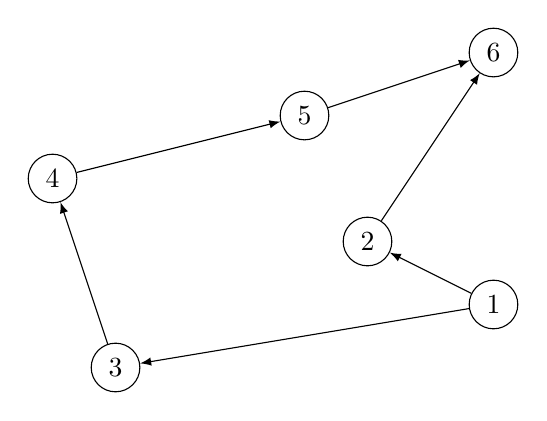
\begin{tikzpicture}
	  [scale=.8,auto=left,every path/.style={>=latex},every node/.style={draw, circle}]
	  \node (n6) at (11,10) {6};
	  \node (n4) at (4,8)  {4};
	  \node (n5) at (8,9)  {5};
	  \node (n1) at (11,6) {1};
	  \node (n2) at (9,7)  {2};
	  \node (n3) at (5,5)  {3};

	  \foreach \from/\to in {n5/n6,n1/n2,n1/n3,n2/n6,n3/n4,n4/n5}
	    \draw[->] (\from) -- (\to);
	\end{tikzpicture}
	\\
\noindent In the figure above, the longest path is $\{v_1, v_3, v_4, v_5, v_6\}$, with length 4. The algorithm given returns $\{v_1, v_2, v_6\}$, which is a path of length 2 $<$ 4.
\end{homeworkSection}
\begin{homeworkSection}{Solution: Design and Reasoning}
\noindent We want a path which maximizes the number of edges, \emph{M}, between nodes $v_1$ and $v_n$. Clearly, the last node and first node must be part of every solution, including the optimal solution. Suppose that an optimal solution \emph{O} exists - then, we can characterize it by performing a case analysis and identifying potential sub-solutions: Since we know that $v_n \in O$, at least one of the nodes leading into $v_n$ must also be in \emph{O}. These $\delta_{in}(v_n)$ nodes form a subset $V_n \subset V$ and their edges terminating form a subset $E_n$. Following this pattern, we can break G into subgraphs $G_i = \{V_i, E_i\}$, where $V_i = \{ v_j \in V | (v_j, v_i) \in E_{out} \}$ and $E_i = \{ (u, v) \in E | v = v_i\}$ with sub-solutions of length $l_i$. If a node $v_i \notin O$, then the subset of edges incident on $v_i$ is also not in \emph{O}, so we can simply ignore those edges and continue searching. If $v_i \in O$, then we search for the sub-path of max length terminating at $v_i$ in the subgraph $G_i$. Then, the max-length path terminating at $v_i$ is $M_i$ with length $l_i$, where $l_i = max(l_{1},...,l_{i-1})+1$.
\end{homeworkSection}
\begin{homeworkSection}{Solution: Implementation}
Like the majority of solutions seen in this chapter, this algorithm stores the max-length of paths terminating at each node in an array called \emph{L} as it iterates through nodes. If we did this recursively, we would begin at the last node. However, we use an iterative solution, in keeping with the style of this chapter:\\
\problemAnswer{ % Answer
\setlength\parindent{25pt}
\noindent Let L be array of size n.\\
\noindent Initialize the array to 0.\\
\noindent For i in 2,...,n:\\
\indent For all j such that $(v_j, v_i) \in$ E:\\
\indent \indent If $L[j] > L[i]-1$,\\
\indent \indent \indent $L[i] = L[j]+1$.\\
\noindent Return L[n].\\
}
\end{homeworkSection}
\begin{homeworkSection}{Solution: Proof and Time Complexity}
\noindent The algorithm stores the max-length of paths terminating at a given node $v_i$. By definition, L[1] = 0. For i = 2, the algorithm correctly computes that L[2] = 1, since L[1] = 0 $>$ -1 = L[2]-1. Let $i > 1$, and suppose by way of induction that the algorithm correctly computes L[i] for all $i < n$. Then, $l_n$ = L[n] = $max(l_{j}, l_{j+1},..., l_{n-1})+1$, as desired. Since the $i^{th}$ node has at most $i-1$ in-edges, the inner loop runs at most $\sum_{i=1}^{n} (n-i) = \frac{n*(n-2)}{2}$ times. Thus, the algorithm is $\mathcal{O}(n^2)$.
\end{homeworkSection}
\end{homeworkProblem}

%----------------------------------------------------------------------------------------
%	PROBLEM 2
%----------------------------------------------------------------------------------------

\begin{homeworkProblem} % Custom section title
\noindent The exercise asks us to write an algorithm that, given a sequence of n supply values (in lbs per week), returns an optimized schedule for the shipment of supplies at minimum overall cost. Cost is either a function of weight or time, depending on the shipping company chosen: Company A charges r dollars per lb, and company B charges c dollars per week for a 4-week (consecutive) contract.
%--------------------------------------------
\begin{homeworkSection}{Solution: Design and Reasoning}
We want to find all 4-subsequences such that $4c < r\sum_{i=k}^{k+4} S_i$. Those are the subsequences that will be shipped via company B. Suppose there is an optimal sequence of companies \emph{O}. Because the supply values must be shipped out sequentially, we know that if B is chosen in the $i^{th}$ week in \emph{O}, then the cost at the $i+4^{th}$ point in time is $c_{i+4} = c_{i-1}+4c$. Similarly, if A chosen in the $i^{th}$ week, the cost at point \emph{i+4} is $c_{i+4} = rs_{i+4}+c_{i-3}$. Thus, when choosing company A or B for the $i^{th}$ week in our schedule, we must minimize $c_i$ such that $c_i = min(4c+c_{i-4}, rs_i+c_{i-1})$.
\end{homeworkSection}
\begin{homeworkSection}{Solution: Implementation}
	\problemAnswer{ % Answer
	\setlength\parindent{25pt}
	\noindent Let C be an array of size n.\\
	\noindent Let S be an array of size n.\\
	\noindent Initialize C to 0.\\
	\noindent For i in 1,...,n:\\
	\indent C[i] = min(4c+C[i-4], r$s_i$+C[i-1]).\\
	\indent If C[i] = 4c+C[i-4],\\
	\indent \indent S[i] = B.\\
	\indent Else, C[i] = r$s_i$+C[i-1],\\
	\indent \indent S[i] = A.\\
	\noindent Return S, C[n].
	}
	\end{homeworkSection}
\begin{homeworkSection}{Solution: Time Complexity}
\noindent Each iteration of the loop assigns a cost equal to $min(4c+c_{i-4}, rs_i+c_{i-1})$ for each week, as desired. The main loop runs each time, and each iteration requires a constant k steps to check for the appropriate minimum cost of the shipping $s_i$. Thus, the algorithm is $\mathcal{O}(n)$.
\end{homeworkSection}

\end{homeworkProblem}

%----------------------------------------------------------------------------------------
%	PROBLEM 3
%----------------------------------------------------------------------------------------

\begin{homeworkProblem}% Roman numerals
A rising trend in stock prices over n days is defined as a k-subsequence of the n prices over $i_k$ days such that the following conditions hold:\\
\setlength\parindent{25pt}
\indent (i). $i_1$ = 1.\\
\indent (ii). $P_i < P_{i+1}$ for each j = 1, 2, ..., k-1.

\begin{homeworkSection}{Counterexample for algorithm 17a:}
\noindent The algorithm fails on the subsequence {2, 4, 3, 4, 5, 7, 6, 7}, returning {2, 4, 5, 7} with length 4 when the correct subsequence is {2, 3, 4, 5, 6, 7} with length 6.
\end{homeworkSection}

\begin{homeworkSection}{Solution: Design and Reasoning}
\noindent Suppose that there is an optimal solution O that returns length $L_k$ for some longest k-subsequence. The subsequence ending at $i_{k-1}$ has length $L_{k-1}$ and consists of the longest rising trend observed from $i_1$ to $i_{k-1}$. Thus, $L_k = L_{k-1}+1$. If a price $P_i \in L_k$, then $P_i < P_j \forall j > i$, thus any $P_{i-1} \in L_k$ must be smaller than $P_i$.
For some $P_i$, we can store the longest subsequence from $P_1$ to $P_i$. Then, $L_{i+1} = L_i + 1$ if $P_{i+1} > P_{i}$. Else, $L_{i+1} = 1+max(L_j) \forall j < i$.
\end{homeworkSection}% Question
\begin{homeworkSection}{Solution: Implementation}
	\problemAnswer{ % Answer
	\setlength\parindent{25pt}
	\noindent Let L be an array of size n, P an array of stock prices.
	\noindent Initialize L[1] = 0, L[i] = -1, i=2,...,n.\\
	\noindent For i in 2,...,n:\\
	\indent If P[i-1] < P[i], L[i] = max(0, L[i-1]+1).\\
	\indent Else, j = i-2, l = 0.\\
	\indent \indent While P[j] < P[i] and j > 1:\\
	\indent \indent \indent l = max(L[j], l).\\
	\indent \indent \indent j = j-1.\\
	\indent \indent L[i] = l.\\
	\noindent Return max(L[1,...,n]).
	}
\end{homeworkSection}% Question
\begin{homeworkSection}{Solution: Proof and Time Complexity}
\noindent We can prove that this algorithm returns a correct solution by induction on i. For i=2, the algorithm returns 1 if $P_1 < P_2$ or else it returns 0. This is the correct length for a subsequence beginning at 1 and ending at 2. Assume that the algorithm returns the correct length for all stocks $P_i$ from 1 to n-1. Then, for the $n^th$ stock, $L[n] = L[n-1]+1$ if $P_n$ is larger than $P_{n-1}$ or 1 + max-length for a subsequence of stocks between 1 and n-2, as desired. The main for loop runs n times, and each iteration i requires \emph{i-2} iterations of the while loop, so this algorithm is $\mathcal{O}(n^2)$.
\end{homeworkSection}% Question
\end{homeworkProblem}

%----------------------------------------------------------------------------------------

%----------------------------------------------------------------------------------------
%	PROBLEM 4
%----------------------------------------------------------------------------------------

\begin{homeworkProblem}
I'm unsure of how to approach this problem. I read the section in the textbook but still feel as though I don't truly understand what I'm being asked, let alone the solution. Hopefully the TA can go over this type of problem during discussion, since it was not covered in lecture.

\end{homeworkProblem}

%----------------------------------------------------------------------------------------
%	PROBLEM 5
%----------------------------------------------------------------------------------------

\begin{homeworkProblem} % Roman numerals

\begin{homeworkSection}{Description} % Section within problem
The exercise asks us to produce an efficient algorithm that computes the number of shortest paths between (v,w) in a weighted graph G with no negative cycles (but possibly negative edge weights).
\end{homeworkSection}


\begin{homeworkSection}{Solution: Reasoning and Implementation} % Section within problem	
Since we have a weighted graph, we can't use BFS, and since we have negative edge weights, we can't use Dijkstra's algorithm. Thus, we must use a modified version of the Bellman-Ford algorithm described in [KT], section 6.9. First, we have to compute the length of the shortest path, which we can do using the algorithm described on [KT] pg 294. Then, we can add an additional for-loop to the algorithm to compute the number of shortest paths from v to w with the desired length.
\\
\\
	\problemAnswer
	{ % Answer
	\setlength\parindent{25pt}
	\noindent Let n = number of nodes in G.\\
	\noindent Array M[0,...,n-1, V].\\
	\noindent Define M[k, v] = 0, M[k, u]=$\infinity$, if u $\neq$ v.\\
	\noindent For i in 1,...,n-1:\\
	\indent For j in 1,...,n:\\
	\indent \indent M[i, j] = min(M[i-1, j-1] + $c_{ij}$).\\
	\noindent P = $min_1^i$(M[i,w]), L=length(P), N=0.\\
	\indent For i in 1,...,n:\\
	\indent \indent If M[P, i] $\leq$ P, N++.\\
	\noindent Return N.
	}
\end{homeworkSection}

\begin{homeworkSection}{Solution: Time Complexity} % Section within problem
The algorithm works in almost exactly the same way as the Bellman-Ford algorithm described in the textbook, with a few modifications that allow us to keep track of the number of shortest paths. The time complexity is $\mathcal{O}(n^3)$, since the inner most for-loop runs $n^2$ times at worst and examines up to n nodes per iteration during construction of the \emph{M} matrix.
\end{homeworkSection}

\end{homeworkProblem}

%----------------------------------------------------------------------------------------

%----------------------------------------------------------------------------------------
\end{document}
